%--------------------------------------------------------------------------------------------------------------------------------------------VPN
\section{Virtual Private Networks }
Una rete privata virtuale consiste in una rete il cui accesso è regolamentato, che si appoggia a un protocollo di trasporto pubblico e condiviso, e che consente di garantire confidenzialità della comunicazione, accesso solo previa autenticazione, integrità dei dati e protezione da alcuni tipi di attacchi, ad esempio Man-in-the-middle o attacco replay.

\subsection{Architetture disponibili}
Una rete VPN può realizzare diversi tipi di collegamenti, per soddisfare esigenze diverse. Nei paragrafi successivi, si andranno ad analizzare i 3 tipi di architetture più comuni:
\begin{itemize}
    \item Gateway-to-Gateway
    \item Host-to-Host
    \item Host-to-Gateway
\end{itemize}

\subsubsection{Gateway-to-Gateway}
Consiste in una VPN che connette in maniera stabile due reti. Questa configurazione permette ad esempio di estendere una rete privata tra diverse location geograficamente separati e distanti a piacere, oppure di garantire a una serie di uffici un accesso sicuro a un data center.

\subsubsection{Host-to-Host}
Questa configurazione è la meno comune. Consiste nello stabilire una comunicazione diretta tra due host, in cui uno fa da server VPN e l'altro da client VPN. Un caso d'uso potrebbe essere un amministratore di sistema che deve fare gestione remota di un apparecchio.

\subsubsection{Host-to-Gateway}
In questa modalità, il risultato che si ottiene è lo stesso che si avrebbe connettendo un host alla rete locale in cui risiede il server VPN.
È usata principalmente per offrire un accesso sicuro da remoto alla rete. Quando l'host vuole instaurare una connessione VPN con il server, gli viene richiesto di autenticarsi.

\subsection{Soluzioni principali}
Tra le soluzioni VPN più comuni troviamo:
\begin{itemize}
    \item Point-to-Point Tunneling Protocol
    \item IP Security Protocol
    \item OpenVPN
    \item Wireguard
    \item Mettere Esempio di Web Based SSL VPN %https://www.firewall.cx/cisco-technical-knowledgebase/cisco-services-tech/342-cisco-web-vpn.html
\end{itemize}



\subsection{Perché soddisfano i requisiti}
Prova di testo di capitolo. Vorrei citare qui tutta l'opera omnia di
%---------------------------------------------------------------------------------------------------------------------------------------------IPSec
% BUONO https://pctempo.com/openvpn-vs-ikev2-vs-pptp-vs-l2tp-ipsec-vs-sstp/

% https://it.wikipedia.org/wiki/IPsec https://github.com/sunknudsen/privacy-guides/blob/master/how-to-self-host-hardened-strongswan-ikev2-ipsec-vpn-server-for-ios-and-macos/README.md 

% 1.	Come è nato
% 2.	Tipo incapsulamento
% 3.	Overhead - byte sprecati per pacchetto
% 4.	Livello a cui lavora
% 5.	Protocolli usati
% 6.	Cifratura usata ? hw o sw, limitata se non aggiorni hw ma più veloce, e il contrario

\section{IPSec}
\subsection{Panoramica}
IPsec is a framework of open standards for ensuring private communications over IP networks which has become the most commonly used network layer security control [11]. IPsec is based on securing Network layer of TCP/IP model. In many environments securing Network layer is a better solution than securing higher Transport or Application layers. It makes a way for network administrators to enforce certain security policies, and also provides a more flexible way in protecting IP information for each packet [11]. Depending on the implementation IPsec can provide a combination of following security measures: confidentiality, integrity, peer authentication, replay protection, traffic analysis protection and access control.

\subsection{Protocolli utilizzati}
As noted earlier, IPsec uses multiple additional protocols to establish a secure connection [11]

\subsubsection{Authentication Header}
Authentication Header (AH) , defined in RFC 4302 [12], provides integrity protection for all packet headers (except few IP header fields) and user authen- tication. Optionally it can provide replay and access protection. AH is not able to encrypt data.

\subsubsection{Encapsulating Security Payload}
Encapsulating Security Payload (ESP) , defined in RFC 4303 [13], has two modes: tunnel and transport. Tunnel mode can provide encryption and integrity protection for an encapsulated IP packet as well as authentication for ESP header, while transport mode can provide encryption and integrity protection for the payload of an IP packet and integrity protection for the ESP header.

\subsubsection{Internet Key Exchange v2}
Ancora del testo---IKE è un acronimo per Internet key exchange ed è il protocollo usato per stabilire una security association nella suite di protocolli IPsec. Questo protocollo è definito in RFC 4306. È un protocollo di livello applicazione e utilizza il protocollo UDP come protocollo di trasporto; la porta su cui viene stabilita la connessione è 500. ---

Internet Key Exchange (IKE) is used to negotiate, create and manage Secu- rity Associations (SA) [11]. SA is a set of rules needed to define the features and security mechanisms for the establishing a IPsec connection. It can be defined manually, however it does not scale well with large-scale VPNs. A more common method is using one of the five possible IKE exchange modes - main, aggres- sive, quick, informational or group. The modes differ in speed and the usage of their cryptographic primitives for establishing a secure connection. IKEv2 is the newest version of IKE, and it improves the protocol in the following ar- eas: clearly defined RFC (RFC 5996 [14]), simplicity, reliable message delivery, protection against Denial of Service (DoS) attacks, and improved usage of IKE with Network Address Translation (NAT) gateways [11].


\subsection{Transport mode vs Tunnel mode}
Ancora del testo

\subsection{Cifratura}
Ancora del testo

\subsection{Autenticazione}
Ancora del testo

\subsection{Implementazioni}
StrongSwan is an open source IPsec implementation for the Linux oper- ating system [18]. Maintained by Andreas Steffen, strongSwan supports features, such as IPv6, Android 4+, X.509 public key certificates, certifi- cate revocation lists, RSA private key storage on smartcards, ability to interoperate with various MS Windows and Mac OS X VPN clients, full implementation of IKEv2 protocol, and much more.

\subsection{Considerazioni}
Ancora del testo
%---------------------------------------------------------------------------------------------------------------------------------------------PPTP
% https://www.ivpn.net/pptp-vs-ipsec-ikev2-vs-openvpn-vs-wireguard/

\section{PPTP}
\subsection{Panoramica}
Si tratta di uno dei più vecchi protocolli VPN in uso ancora oggi, ma in quanto tale ha alcune gravi criticità date dall'età. Ad esempio, la crittografia a 128 bit e il protocollo usato per l'autenticazione (MS-CHAP) contenente note vulnerabilità lo rendono ormai un protocollo insicuro, da evitare se le informazioni che transitano sono sensibili.
Tuttavia, è estremamente semplice da configurare e il più veloce dal punto di vista prestazionale, il che lo rende ideale per usi quali streaming video o l'utilizzo di VPN su terminali con potenze di calcolo estremamente limitate.
È stato sviluppato da Microsoft nel 1999 \cite[RFC2637]{RFC2637} e lavora instaurando un canale di controllo tra i due peers sulla porta 1723 TCP e un tunnel GRE su cui transitano effettivamente i dati.

\subsection{Protocolli utilizzati}
\subsubsection{Generic Routing Encapsulation}
GRE è un protocollo di tunneling sviluppato da Cisco Systems che può incapsulare un'ampia varietà di protocolli di livello di rete all'interno di collegamenti Point-to-Point o Point-to-Multipoint virtuali su una rete IP.

\subsection{Cifratura}
PPTP non specifica nessuna

\subsection{Autenticazione}
Ancora del testo

\subsection{Considerazioni}
Ancora del testo

%----------------------------------------------------------------------------------------------------------------------------------------------OpenVPN
% https://en.wikipedia.org/wiki/OpenVPN 
\section{OpenVPN}
\subsection{Panoramica}
OpenVPN è una VPN SSL che permette di incanalare tutto il traffico di una sottorete attraverso una unica porta UDP o TCP, e fa affidamento su OpenSSL. Come le altre soluzioni VPN, OpenVPN servizi essenziali di sicurezza quali autenticazione, cifratura, integrità dei dati e controllo degli accessi.
Supporta due modalità di lavoro, routing e bridging:
\begin{itemize}
    \item[Routing] consiste nell'interconnessione di due sottoreti indipendenti, dove il server VPN (generalmente installato sul router) inoltra i pacchetti all'indirizzo IP specificato in fase di configurazione. Si tratta quindi di un collegamento a livello 3 del modello OSI.
    \item[Bridging] è una modalità che lavora esclusivamente all'interno di una sottorete; il funzionamento è analogo a quello di uno switch ethernet fisico.
\end{itemize}

OpenVPN è una soluzione che lavora in user space, dunque l'overhead generato è maggiore in quanto sono necessarie molteplici copie dei pacchetti affiché siano trasferiti dal kernel space allo user space. Supporta l'intero insieme delle funzionalità di TLS, necessitando di una ampia code base, mostrando un maggior potenziale a soffrire di vulnerabilità.

\subsection{Protocolli utilizzati}
Come precedentemente acccennato, OpenVPN usa la libreria di OpenSSL, che implementa il protocollo Transport Layer Security, progettato per offrire una connessione sicura attraverso una rete non sicura.
A differenza del puro TLS, OpenVPN offre all'utente la possibilità di utilizzare una pre-shared key per generare quel che è noto come HMAC firewall, che autentica tutta la sequenza di handshake TLS.

Essendo UDP un protocolllo non connesso, i pacchetti IP criptati e firmati che sono incanalati tramite UDP, non hanno nessuna garanzia di affidabilità. L'affidabilità necessaria per una sicura autenticazione è garantita, però, dal protocollo TLS che utlizza TCP come protocollo di trasporto.
È importante notare che il canale dati e il canale di controllo transitano all'interno dello stesso tunnel UDP (o TCP). L'incapsulamento dei pacchetti è descritto dal seguente diagramma.

\begin{figure}
    \centering
    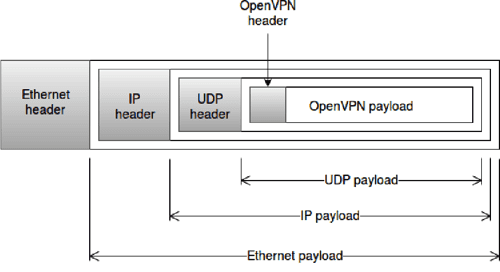
\includegraphics[width=8cm]{figure/OVPN_packet.png}
    \caption{Dettaglio di un pacchetto OpenVPN}
\end{figure}

La struttura mostrata si applica a tutti i pacchetti OpenVPN; tuttavia, differenti pacchetti avranno differenti payloads.


\subsubsection{Secure Socket Layer/Transport Layer Security VPNs}
Il protocollo Transport Layes Security, originariamente noto come Secure Socket Layer, è un protocollo progettato per garantire una connessione sicura attraverso una rete non sicura. TLS permette autenticazione di client e server, integrità dei dati e confidenzialità. Per l'autenticazione usa i certificati X.509 \cite[RFC5280]{RFC5280} con una crittografia asimmetrica e si occupa di negoziare una chiave di sessione simmetrica.

One advantage of SSL VPNs over an IPsec VPNs is that SSL VPNs can connect to more restricted environments where NAT (Network Address Translation) or strict firewall rules are used. The reason for this is because most organizations do not filter the traffic on the TCP port 443, as it is usually used for employees to securely access Internet. For instance, OpenVPN, SSL- based VPN, uses UDP Port 1194 for secure data transmission. However, in the case that port is filtered, OpenVPN can also make use TCP port 443. The advantages of using UDP as a transport protocol are discussed at the beginning of the Chapter 4.
There are two primary types of SSL VPNs, namely SSL portal VPNs and SSL tunnel VPNs [15].
• SSL portal VPN works over a single network port, namely TCP 443 and acts as a Transport layer VPN. It allows users to connect with most web browsers to access web related content.
• SSL tunnel VPN is used to access multiple network services through a tunnel that is running under SSL. The main difference from portal SSL VPNs is that tunnel SSL VPNs allow accessing multiple network services, including applications and protocols that are not web-based. The require- ment for SSL tunnel VPN is that it must be able to handle different active content like Java, JavaScript, Flash, ActiveX [15]. Being able to use more services, this tunnel has more capabilities compared to a portal type VPNs, but it may prevent some users from being able to connect to VPN. The SSL VPN tunnels are created in SSL, but just like in IPsec tunnels, IP traffic is fully protected by the tunnel [15].

\subsection{TCP vs UDP}

TCP is the main protocol in TCP/IP networks. The IP protocol process data packets while TCP allow two hosts to exchange data streams and establish a connection. TCP guarantees that packets will arrive their destination in the same order in which they were sent [7].
UDP provides unreliable, minimum, best-effort, message delivery to upper-layer protocols and applications. UDP do not setup a permanent connection between two end points [8].
IV. COMPARISON BETWEEN TCP AND UDP
The adjustments between TCP and UDP regardless of VPN usage is always said to be the same: Speed is sacrifice for reliability as UDP is connectionless and the server sending the data theoretically does not ensure if it reaches the des- tination or not. TCP is a connection-oriented protocol [9], which implies that end-to-end communications is set up using handshaking. Once the connection is established, data can be transferred bi-directionally over the link. UDP is a connec- tionless protocol and therefore less complex message based [10] when compared to TCP, which includes that the point-to- point connection is not dedicated and data is transferred uni- directional from the source to its destination without checking whether the receiver is active. TCP regulate retransmission, message acknowledgment, and timeout [11]. TCP deliver lost messages along the way upon multiple attempts. In TCP, there is no missing data, and if ever there are multiple timeouts, the connection is dropped. When a UDP message is sent there is no guarantee that the message will reach its destination; it could get drop along the way. There is no retransmission, timeout and acknowledgment. When two data packets are sent in sequence, the first message will reach the destination first. When data segments arrive in the wrong order, TCP buffers hold the data until all data are re-ordered before being transmitted; when using UDP the order in which messages arrive cannot be predicted.
The TCP protocol has extensive algorithms to ensure correct delivery of the data. Having two TCP connections stacked together will thus force the algorithms of both TCP con- nections to work in parallel [12]. TCP was not designed to work this way and problems are likely to occur in different situations. The retransmission problems, TCP meltdown and double retransmit, are problems caused by tunneling TCP in TCP. The problems can occur when both of the stacked con- nections are retransmitting packets. In previous work, related to TCP in TCP tunneling, it is not entirely clear, how severe the retransmission problems really are. TCP protocol suite allows automatic recovery of any dropped or lost data even if a host goes down in the network. When TCP packets are transmitted from one end to a remote end across the network, the data packets are reordered in the same sequence created by the sender. The protocol notifies when segments of the data stream have been corrupted, reordered, discarded or duplicated by the network [11]. TCP is a reliable protocol as the sender can retransmit damaged segments. However retransmission creates latency.
TCP was designed to make an efficient protocol with little overhead, a protocol set having a basic amount of ’extra’ data being transferred. This extra data is named as overhead,
and they package the data that needs to be transferred. TCP tunnel is a technology that combines and transmits packets sent between end hosts as a single TCP connection. When using a TCP tunnel, the fairness among aggregated flows can be improved and several protocols can be transparently transmitted through a firewall

\subsection{Cifratura}
Ancora del testo

\subsection{Autenticazione}
In contrast to pre-share static key mode, TLS mode uses TLS protocol to authen- ticate, establish secure channel and exchange the symmetric tunnel session key between peers.
Just like in pre-shared static key mode, session key is used to en- crypt the data tunnel, however, the authentication and symmetric key exchange take place using TLS protocol.
This not only provides an automatic and secure way of distributing symmetric keys, but also a way to renew the symmetric key at any point during the communication.
The aforementioned aspect of the TLS mode provides the Perfect Forward Secrecy, which is not present in pre-shared static key mode.
The structure of the tunnel session key derivation TLS packet, as shown in Wireshark, can be seen in Fig. 4.
The transfer of tunnel session keys are encrypted and carried inside the TLS Record layer, so it cannot be decrypted without the proper TLS certificates. The two main steps in this protocol are shown below.
1. Negotiation of the TLS connection. Both sides of the connection are au- thenticated by exchanging certificates and verifying the certificate of the opposing side. If the authentication is successful, the protocol proceeds wit the step two. Otherwise, the connection is terminated.
2. Tunnel session keys are negotiated over the already established secure TLS channel. The tunnel session key derivation TLS packet structure depends on the OpenVPN key method being used. TLS mode supports two key methods, which are described below.
If the first key method is used, then the tunnel session keys are derived from OpenSSL cryptographic library RAND bytes function.
The tunnel session key derivation TLS packet structure is shown in Tab. 3.
(b) If the second key method is used, (default in the OpenVPN 2.0+), then the tunnel session keys are derived from the RAND bytes func- tion passed through the TLS pseudo-random function (TLS PRF).
In order to successfully construct a OpenVPN client, it is important to un- derstand the key differences explained in this chapter between the TLS modes, key methods and their respective packet structures.

\subsection{Misure di sicurezza aggiuntive}
Ancora del testo
OpenVPN offers various internal security features. It has up to 256-bit encryption through the OpenSSL library, although some service providers may offer lower rates, effectively providing some of the fastest VPN available to consumers. It runs in userspace instead of requiring IP stack (therefore kernel) operation. OpenVPN has the ability to drop root privileges, use mlockall to prevent swapping sensitive data to disk, enter a chroot jail after initialization, and apply a SELinux context after initialization.

OpenVPN runs a custom security protocol based on SSL and TLS, rather than supporting IKE, IPsec, L2TP or PPTP.

OpenVPN offers support of smart cards via PKCS 11-based cryptographic tokens.
\subsection{Considerazioni}
Ancora del testo

%--------------------------------------------------------------------------------------------------------------------------------------------Wireguard
\section{WireGuard}
\subsection{Panoramica}
In Linux, the standard solution for encrypted tunnels is IPsec, which uses the Linux transform (“xfrm”) layer. Users fill in a kernel structure determining which ciphersuite and key, or other transforms such as compression, to use for which selector of packets traversing the subsystem. Generally a user space daemon is responsible for updating these data structures based on the results of a key exchange, generally done with IKEv2 [13], itself a complicated protocol with much choice and malleability. The complexity, as well as the sheer amount of code, of this solution is considerable. Administrators have a completely separate set of firewalling semantics and secure labeling for IPsec packets. While separating the key exchange layer from the transport encryption— or transformation—layer is a wise separation from a semantic viewpoint, and similarly while separating the transformation layer from the interface layer is correct from a networking viewpoint, this strictly correct layering approach increases complexity and makes correct implementation and deployment prohibitive.
WireGuard does away with these layering separations. Instead of the complexity of IPsec and the xfrm layers, WireGuard simply gives a virtual interface—wg0 for example—which can then be administered using the standard ip(8) and ifconfig(8) utilities. After configuring the interface with a private key (and optionally a pre-shared symmetric key as explained in section 5.2) and the various public keys of peers with whom it will communicate securely, the tunnel simply works. Key exchanges, connections, disconnections, reconnections, discovery, and so forth happen behind the scenes transparently and reliably, and the administrator does not need to worry about these details. In other words, from the perspective of administration, the WireGuard interface appears to be stateless. Firewall rules can then be configured using the ordinary infrastructure for firewalling interfaces, with the guarantee that packets coming from a WireGuard interface will be authenticated and encrypted. Simple and straightforward, WireGuard is much less prone to catastrophic failure and misconfiguration than IPsec. It is important to stress, however, that the layering of IPsec is correct and sound; everything is in the right place with IPsec, to academic perfection. But, as often happens with correctness of abstraction, there is a profound lack of usability, and a verifiably safe implementation is very difficult to achieve. WireGuard, in contrast, starts from the basis of flawed layering violations and then attempts to rectify the issues arising from this conflation using practical engineering solutions and cryptographic techniques that solve real world problems.

For key distribution, WireGuard draws inspiration from OpenSSH, for which common uses include a very simple approach toward key management. Through a diverse set of out-of-band mechanisms, two peers generally exchange their static public keys. Sometimes it is simple as PGP-signed email, and other times it is a complicated key distribution mechanism using LDAP and certificate authorities. Importantly, for the most part OpenSSH key distribution is entirely agnostic. WireGuard follows suit. Two WireGuard peers exchange their public keys through some unspecified mechanism, and afterward they are able to communicate. In other words, WireGuard's attitude toward key distribution is that this is the wrong layer to address that particular problem, and so the interface is simple enough that any key distribution solution can be used with it. As an additional advantage, public keys are only 32 bytes long and can be easily represented in Base64 encoding in 44 characters, which is useful for transferring keys through a variety of different mediums.
Finally, WireGuard is cryptographically opinionated. It intentionally lacks cipher and protocol agility. If holes are found in the underlying primitives, all endpoints will be required to update. As shown by the continuing torrent of SSL/TLS vulnerabilities, cipher agility increases complexity monumentally. WireGuard uses a variant of Trevor Perrin's Noise [23]—which during its development received quite a bit of input from the authors of this paper for the purposes of being used in WireGuard—for a 1-RTT key exchange, with Curve25519 [5] for ECDH, HKDF [15] for expansion of ECDH results, RFC7539 [17]'s construction of ChaCha20 [3] and Poly1305 [8] for authenticated encryption, and BLAKE2s [2] for hashing. It has built-in protection against denial of service attacks, using a new crypto-cookie mechanism for IP address attributability.
Similarly opinionated, WireGuard is layer 3-only; as explained below in section 2, this is the cleanest approach for ensuring authenticity and attributability of the packets. The autqwhors believe that layer 3 is the correct way for bridging multiple IP networks, and the imposition of this onto WireGuard allows for many simplifications,
3
resulting in a cleaner and more easily implemented protocol. It supports layer 3 for both IPv4 and IPv6, and can encapsulate v4-in-v6 as well as v6-in-v4.
WireGuard puts together these principles, focusing on simplicity and an auditable codebase, while still being extremely high-speed and suitable for a modicum of environments. By combining the key exchange and the layer 3 transport encryption into one mechanism and using a virtual interface rather than a transform layer, WireGuard indeed breaks traditional layering principles, in pursuit of a solid engineering solution that is both more practical and more secure. Along the way, it employs several novel cryptographic and systems solutions to achieve its goals.

\subsection{Protocolli utilizzati}
Ancora del testo

\subsubsection{Something}
Ancora del testo

\subsection{TCP vs UDP}
Ancora del testo

\subsection{Cifratura}
Ancora del testo

\subsection{Autenticazione}
Ancora del testo

\subsection{Considerazioni}
Ancora del testo